\chapter{Automation Mixing}
\label{chap:automation}

\classquote{穷则变，变则通，通则久。}{《周易·系辞下》 / The Book of Changes, "Xi Ci II"}{Translation: When it is exhausted, it changes; having changed, it passes through; having passed through, it lasts. Note: automation changes faders and parameters over song time; it is not a static switch.}

Static mixing answers ``where should the fader sit for the whole song?'' Automation answers ``where should it sit at bar 5?'' In Yeban, automation is not a switch inside a plug-in. It is a set of curves attached to each track: every point stores a tick and a value, and playback or export evaluates the curve through one model entry point. The resulting value replaces the target's static value; it is not added to it. This chapter documents only the targets, lanes, read/write flags and edit entry points that exist on the live tip. Missing pieces are listed at the end.

\section{The layers of automation}

An automation lane is defined by three things: a target, points, and read/write state. The target answers ``what is controlled'', the points answer ``when and how much'', and the read/write state answers ``should playback use it, and should recording write it''.

\begin{table}[htbp]
\centering
\small
\begin{tabular}{@{}p{0.18\linewidth}p{0.25\linewidth}p{0.19\linewidth}p{0.27\linewidth}@{}}
\hline
Target variant & Addressing & Unit and nominal display range & Value used without automation \\
\hline
\texttt{TrackVolume} & track ID & dB, $-60$--$+12$ & static \texttt{volume\_db} \\
\texttt{TrackPan} & track ID & bipolar, $-1$--$+1$ & static \texttt{pan} \\
\texttt{SendGain} & track ID + routing edge ID & dB, $-60$--$+12$ & edge \texttt{gain\_db}; absent = unity 0 dB \\
\texttt{DeviceParam} & track ID + device slot + parameter index & native parameter unit; the model declares no range & current device parameter value \\
\texttt{Macro} & track ID + macro index & normalized, $0$--$1$ & current macro position \\
\texttt{MidiCc} & track ID + controller number & raw 7-bit value, $0$--$127$ & controller default 0 \\
\hline
\end{tabular}
\caption{The six automation targets in Yeban; this chapter focuses on the first four}
\label{tab:automation-targets}
\end{table}

``Nominal display range'' is only the default vertical axis. It is not a write clamp: the model only requires finite point values, and a curve may sit outside the displayed range while the UI clamps only the pixel position. Do not read $-60$--$+12$ as ``values outside this range are rejected''.

\begin{center}
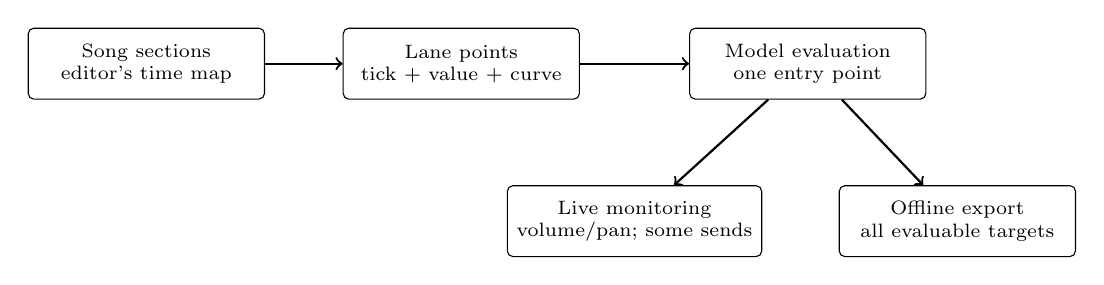
\begin{tikzpicture}[
  box/.style={draw, rounded corners=2pt, minimum width=30mm, minimum height=9mm, align=center, font=\scriptsize},
  arrow/.style={->, thick}
]
  \node[box] (sec) at (0,0) {Song sections\\editor's time map};
  \node[box] (pts) at (4.0,0) {Lane points\\tick + value + curve};
  \node[box] (eval) at (8.4,0) {Model evaluation\\one entry point};
  \node[box] (live) at (6.2,-2.0) {Live monitoring\\volume/pan; some sends};
  \node[box] (off) at (10.3,-2.0) {Offline export\\all evaluable targets};
  \draw[arrow] (sec) -- (pts);
  \draw[arrow] (pts) -- (eval);
  \draw[arrow] (eval) -- (live);
  \draw[arrow] (eval) -- (off);
\end{tikzpicture}
\end{center}

A song section is not a container for automation. Yeban has a section entity, but automation lanes only know ticks on a track. Moving, copying or editing a section does not move the curves. To write ``lighter in the verse, lifted in the chorus'', place points at the bar positions yourself.

\section{How lanes are displayed}

In the arrangement view a track can have several automation lanes. Multiple lanes on one track divide the track row into equal bands in a fixed target order; one target gets one band, and bands do not overlap. Lanes are visible by default. \texttt{Cmd/\allowbreak Ctrl+Shift+A} or \emph{View $\rightarrow$ Show/Hide Automation Lanes} toggles them. The menu label says ``(A)'', but the actual binding includes \texttt{Shift}; pressing bare \texttt{A} does not toggle it.

\begin{table}[htbp]
\centering
\small
\begin{tabular}{@{}p{0.24\linewidth}p{0.60\linewidth}@{}}
\hline
UI element & Fact \\
\hline
Lane label & volume shows ``Volume'', pan shows ``Pan'', send shows ``Send <routing-edge ID>'', device parameter shows the parameter name, macro shows the macro name, MIDI CC shows ``CC <number>'' \\
Read/write badge & read-off shows ``Read off''; a non-\texttt{Off} write mode shows ``$\bullet$ Write/Touch/Latch''; both can appear together \\
Curve colour & bright when read is on; dim when read is off, but the points remain \\
Master bus & lanes on the master-bus track are not drawn in the arrangement; master mixing stays on the console strip \\
Empty lane & a lane with no points is not persisted; the UI draws only lanes that already exist in the project \\
\hline
\end{tabular}
\caption{How automation lanes are displayed}
\label{tab:automation-display}
\end{table}

\screenshot{automation-lane-overview}{Arrangement view with several automation lanes visible, including volume, pan and device-parameter bands with read/write badges}

Clicking a lane band adds or edits a point at that position: the horizontal position becomes a tick, the vertical position becomes a value in the lane's effective display range, and a new point defaults to linear. If an existing point lies within 8 pixels of the click, its value is updated and its original curve and identity are preserved; a second point at the same tick is not created. This click entry point can only edit points on an existing lane. It cannot create a lane, drag a point, delete a point, or change a curve shape.

\begin{table}[htbp]
\centering
\small
\begin{tabular}{@{}p{0.20\linewidth}p{0.24\linewidth}p{0.46\linewidth}@{}}
\hline
Action & Entry point & Boundary \\
\hline
Show/hide & \texttt{Cmd/\allowbreak Ctrl+Shift+A}; View menu & visible by default; no ``selected track only'' filter \\
Add/edit point & click inside a lane band & existing lanes only; within 8 px counts as the same point; new point is linear \\
Delete point & no UI entry & use MCP \texttt{removeAutomationPoint} \\
Change curve & no UI entry & write the point's \texttt{curve} through MCP, or edit project JSON \\
Create lane & no UI entry & write the first point (MCP \texttt{yeban\_edit\_automation}) or edit project JSON \\
Read/write flags & no UI entry & badges are display-only; change attributes through MCP \texttt{set\allowbreak Automation\allowbreak Lane} \\
\hline
\end{tabular}
\caption{UI edit entry points for automation points}
\label{tab:automation-edit-entry}
\end{table}

\screenshot{automation-point-edit}{A point added by clicking inside a lane band, with its curve and read/write badge visible}

\section{Points, curves and evaluation}

Yeban uses an integer clock at 960 PPQ, not samples or floating-point seconds. Common conversions:

\begin{table}[htbp]
\centering
\small
\begin{tabular}{@{}lll@{}}
\hline
Duration & ticks & Position in 4/4 \\
\hline
Quarter note (one beat) & 960 & one bar = four beats = 3{,}840 ticks \\
Sixteenth note & 240 & one bar = sixteen sixteenths \\
One bar & 3{,}840 & eight bars = 30{,}720 ticks \\
\hline
\end{tabular}
\caption{Tick conversions for automation points}
\label{tab:automation-ticks}
\end{table}

Between two adjacent points the value is interpolated using the left point's curve. A curve only changes the shape towards the next point; it does not change the endpoint values. All four curves hit both endpoints exactly and do not overshoot:

\begin{table}[htbp]
\centering
\small
\begin{tabular}{@{}lll@{}}
\hline
Serialized name & Normalized weight $u(t)$ & Feel/use \\
\hline
\texttt{Linear} & $t$ & constant-speed fader; most common \\
\texttt{Exponential} & $t^2$ & slow then fast; ``lift at the end'' \\
\texttt{Logarithmic} & $t(2-t)$ & fast then slow; ``reach the value, then hold'' \\
\texttt{SCurve} & $t^2(3-2t)$ & slow at both ends, fast in the middle; section hand-offs \\
\hline
\end{tabular}
\caption{Automation curves; $t$ is the normalized position between two adjacent points}
\label{tab:automation-curves}
\end{table}

Boundary rules:

\begin{itemize}
  \item Before the first point the first value is held; after the last point the last value is held. There is no extrapolation.
  \item An empty lane has no automation value; playback and export fall back to the static value.
  \item If several points share a tick, the point with the largest point ID wins. The UI updates an existing point, so normal editing does not create duplicates at one tick.
  \item A value outside the display range is kept by the model; the UI clamps only the pixel position. Do not infer ``the value was clamped'' from a curve that touches the top of the band.
\end{itemize}

\section{Read switch and write modes}

Each lane has two independent states: \texttt{readEnabled} and \texttt{writeMode}. Read is on by default. Turning it off makes the evaluation entry point return ``no automation value''; playback and export fall back to the static value. The curve remains, but it no longer applies. Write defaults to \texttt{Off}. It is not a record button; it is a gate stored in the document.

\begin{table}[htbp]
\centering
\small
\begin{tabular}{@{}p{0.14\linewidth}p{0.30\linewidth}p{0.44\linewidth}@{}}
\hline
Write mode & Designed meaning & Current implementation \\
\hline
\texttt{Off} & do not record & gate closed; no gesture writes a point \\
\texttt{Write} & write whenever the parameter changes during playback & only writes one point on release of a volume/pan/EQ-low-gain gesture; no ``write while playing'' \\
\texttt{Touch} & write only while the control is touched; stop on release & same release path as \texttt{Write}; no extra branch \\
\texttt{Latch} & keep writing until an explicit stop & same release path as \texttt{Write}; no ``latch until stop'' \\
\hline
\end{tabular}
\caption{Designed meaning of the four write modes and the current implementation; the three non-\texttt{Off} modes are not yet separated}
\label{tab:automation-write-modes}
\end{table}

The UI currently paints read/write state as a badge only. There is no switch, record arm, or mode selector. To change \texttt{readEnabled}, \texttt{writeMode} or an explicit \texttt{domain}, use MCP \texttt{yeban\_edit\_notes} with \texttt{kind: "set\allowbreak Automation\allowbreak Lane"} in \texttt{ops}; to remove the whole lane, use \texttt{remove: true} in the same shape. A lane cannot be created empty: the model refuses to persist the implicit shape ``no points, read on, Off, no override''. Write the first point through \texttt{yeban\_edit\_automation}; the lane appears with the point, then its attributes can be changed.

\subsection{Recording actually writes one point}

Automation recording happens only during playback and only on gesture release. Exactly three gestures currently write a point:

\begin{enumerate}
  \item the mixer track fader (\texttt{TrackVolume});
  \item the mixer track pan control (\texttt{TrackPan});
  \item the device-rack EQ low-shelf gain (\texttt{DeviceParam}, only the EQ low-gain parameter).
\end{enumerate}

On release the current playhead tick is captured and one point is written. Intermediate values during the drag do not form a curve. Press-and-release without movement, dragging back to the original value, stopped playback, a missing lane, and \texttt{writeMode: Off} all write nothing. Send-gain sliders, macros and MIDI CC have no automatic recording path. The send-gain slider changes the routing edge gain; it does not write a \texttt{SendGain} point.

So in the current build the practical meaning of a write mode is ``does this lane allow one point to be written on release'', not four distinct recording behaviours. For a continuous curve, place points by clicking or write them in a batch through MCP.

\section{Writing the four main targets}

\subsection{Volume}

\texttt{TrackVolume} values are absolute dB, not an offset from the fader. When automation exists, the static \texttt{volume\_db} is replaced by the curve; only without automation is the static value used. If the whole song should sit near $-6$ dB, write $-6$ on the curve as well; do not write $0$ and expect it to add to the fader.

Section use: pull down in the verse, restore in the chorus, fade in the outro. Example over eight bars in 4/4 (30{,}720 ticks):

\begin{table}[htbp]
\centering
\small
\begin{tabular}{@{}llll@{}}
\hline
Tick & Bar & Value & Intent \\
\hline
0 & 1 & $-18$ dB & intro starts very low \\
7{,}680 & 3 & $-6$ dB & verse enters \\
15{,}360 & 5 & $0$ dB & chorus at full fader \\
23{,}040 & 7 & $0$ dB & hold \\
30{,}720 & 9 (end) & $-12$ dB & outro pulls back \\
\hline
\end{tabular}
\caption{Volume automation example; values are absolute dB}
\label{tab:automation-volume-recipe}
\end{table}

\subsection{Pan}

\texttt{TrackPan} values are absolute positions from $-1$ to $+1$. They use the pan law and the ``centre identity'' rule from Chapter 7: at $0$ both channels are multiplied by 1; as soon as the value leaves centre it falls onto the selected law. The default $-3$ dB law has a 3.01 dB step between centre and the smallest non-zero value. Automating from $0$ towards $0.6$ therefore produces that step as the curve leaves centre; do not use it for a seamless spread from the middle. To avoid the step, either stay at centre for the section or start from a non-zero value and never cross $0$.

Example: keep centre in the verse, spread the stereo material to $\pm0.6$ in the chorus, return to centre in the outro:

\begin{table}[htbp]
\centering
\small
\begin{tabular}{@{}llll@{}}
\hline
Tick & Bar & Value & Intent \\
\hline
0 & 1 & $0$ & intro centred \\
7{,}680 & 3 & $0$ & verse still centred \\
15{,}360 & 5 & $+0.6$ & chorus spreads right \\
23{,}040 & 7 & $+0.6$ & hold \\
30{,}720 & 9 (end) & $0$ & return to centre \\
\hline
\end{tabular}
\caption{Pan automation example; spread in the chorus, return to centre in the outro}
\label{tab:automation-pan-recipe}
\end{table}

If the source is mono, pan automation only changes the left/right distribution; it does not create new stereo information. Width still belongs to the channel strip's M/S stage (Chapter 7).

\subsection{Sends}

\texttt{SendGain} addresses a routing edge, not ``send number three''. The send row in the UI does not show the edge ID; the lane label shows ``Send <edge ID>''. Read the \texttt{edgeId} from a project query or the project JSON. The value is the edge's absolute gain in dB, not an offset from the static send. When the edge's \texttt{gain\_db} is \texttt{None}, the static value is unity 0 dB. If the static send is $-6$ dB, the first curve point must also be $-6$; otherwise enabling automation jumps the send to 0 dB.

Example: hold $-6$ dB in the verse, make a short $+3$ dB push on the first chorus beat, then return to $-6$:

\begin{table}[htbp]
\centering
\small
\begin{tabular}{@{}llll@{}}
\hline
Tick & Bar & Value & Intent \\
\hline
0 & 1 & $-6$ dB & match the static send \\
15{,}360 & 5 & $-6$ dB & chorus start still held \\
17{,}280 & 5.5 & $-3$ dB & short push \\
19{,}200 & 6 & $-6$ dB & back to the static send \\
30{,}720 & 9 (end) & $-6$ dB & hold \\
\hline
\end{tabular}
\caption{Send-gain automation example; values are absolute dB}
\label{tab:automation-send-recipe}
\end{table}

The send-gain slider does not write a \texttt{SendGain} point; the curve above must be placed by clicking a lane or through MCP. The live result depends on whether the edge actually carries audio. Edges with a live landing apply in monitoring; edges that are missing, sidechain-only, sourced from a bus, or sourced from a non-renderable track apply only in offline export.

\subsection{Effects}

\texttt{DeviceParam} addresses ``the parameter at device slot N, parameter index M''. Values are in the parameter's native unit; the model declares no generic range. The vertical axis either uses an explicit lane \texttt{domain} or adapts to the curve's minimum and maximum. In the UI only the EQ low-shelf gain has a draggable parameter-automation entry; other device parameters can only be written through MCP.

Example: EQ low-shelf gain (parameter range $-18$--$+18$ dB, default 0 dB) slightly cut in the verse, slightly boosted in the chorus:

\begin{table}[htbp]
\centering
\small
\begin{tabular}{@{}llll@{}}
\hline
Tick & Bar & Value & Intent \\
\hline
0 & 1 & $-2$ dB & verse slightly thinner \\
15{,}360 & 5 & $-2$ dB & held before the chorus \\
17{,}280 & 5.5 & $+3$ dB & lift the low shelf in the chorus \\
23{,}040 & 7 & $+3$ dB & hold \\
30{,}720 & 9 (end) & $-2$ dB & return to the verse value \\
\hline
\end{tabular}
\caption{EQ low-shelf automation example; values are in the parameter's native dB}
\label{tab:automation-device-recipe}
\end{table}

\screenshot{automation-device-param}{EQ low-shelf gain in the device rack and the matching device-parameter lane; both use the same slot index}

A device-parameter lane stores a slot index, not a device identity. Inserting or deleting a device before the target makes the same slot point at another device's parameter with the same index. Yeban has no stable \texttt{device\_id} addressing for this lane. After changing the device chain, re-check the lane's landing point.

\section{Designing curves by song section}

Translate ``section'' into a tick range, then decide which target carries each change. Do not pile everything onto volume:

\begin{table}[htbp]
\centering
\small
\begin{tabular}{@{}p{0.14\linewidth}p{0.18\linewidth}p{0.24\linewidth}p{0.30\linewidth}@{}}
\hline
Section & Tick range & Main target & Shape \\
\hline
Intro & 0--7{,}680 & volume & $-18$ to $-6$, linear or S-curve \\
Verse & 7{,}680--15{,}360 & volume, pan & volume $-6$; pan stays centred \\
Chorus & 15{,}360--23{,}040 & volume, send, effect & volume 0; short send push; small EQ low-shelf lift \\
Outro & 23{,}040--30{,}720 & volume, pan & volume back to $-12$; pan back to centre \\
\hline
\end{tabular}
\caption{Automation allocation for an eight-bar section plan}
\label{tab:automation-section-plan}
\end{table}

Workflow:

\begin{enumerate}
  \item Set the static values first: fader, pan, send amount and device parameter are the ``no automation'' baseline.
  \item To create a lane, write the first point through MCP so the lane exists; then set read/write and display domain with \texttt{set\allowbreak Automation\allowbreak Lane}.
  \item In the arrangement view use \texttt{Cmd/\allowbreak Ctrl+Shift+A} to confirm the lane is visible; click points, or write a batch through MCP.
  \item To record, confirm the lane's \texttt{writeMode} is not \texttt{Off}, start playback, drag the fader/pan/EQ low shelf, and release to write one point.
  \item Read back through \texttt{yeban\_edit\_automation} with \texttt{ticks}; check whether \texttt{source} is \texttt{automation} or \texttt{static}.
  \item Before export confirm the read switch is on; a lane that is off does not apply in export either.
\end{enumerate}

Live monitoring and offline export do not have the same landing points. Keep them separate:

\begin{table}[htbp]
\centering
\small
\begin{tabular}{@{}p{0.22\linewidth}p{0.26\linewidth}p{0.42\linewidth}@{}}
\hline
Target & Live monitoring & Offline export \\
\hline
\texttt{TrackVolume} & applies & applies \\
\texttt{TrackPan} & applies & applies \\
\texttt{SendGain} & applies when the edge carries audio & applies; an edge without a live landing applies only in export \\
\texttt{DeviceParam} & only \texttt{output\_gain\_db} on the channel-strip source applies & insert-chain scalar parameters apply; unknown names do not \\
\texttt{Macro} & does not apply & does not apply \\
\texttt{MidiCc} & does not apply & applies \\
\hline
\end{tabular}
\caption{Where automation lands in monitoring and export}
\label{tab:automation-apply}
\end{table}

This means ``I turned the EQ low shelf while monitoring and recorded a point'' does not mean ``I heard the EQ change''. The EQ low shelf is a \texttt{DeviceParam}; the live path has no slot for it. The point is written to the project, but monitoring does not execute it; export does. Do not judge this curve by monitoring alone; render at least once to check it.

\section{Not yet provided, and boundaries}

\begin{table}[htbp]
\centering
\small
\begin{tabular}{@{}p{0.36\linewidth}p{0.54\linewidth}@{}}
\hline
Request & Current state in Yeban \\
\hline
Create/delete lanes in the UI & only by writing a point or editing the project; no ``add automation target'' menu \\
Drag points, marquee-select, batch delete & none; clicking only adds/edits one point \\
Change point curve & none; clicking preserves the curve, new points are linear \\
Read/write switches and mode selector & none; badges are read-only, attributes change through MCP \\
\texttt{Write}/\texttt{Touch}/\texttt{Latch} separation & none; all three non-\texttt{Off} modes write one point on release \\
Continuous fader recording & none; one release writes one point \\
Send-gain slider recording & none; the slider only changes the static routing gain \\
Macro/MIDI CC recording & none \\
Section-level automation container & none; curves live on the track's tick axis and do not move with sections \\
Master-bus lane visualisation & the arrangement does not draw master-bus lanes \\
Stable device-parameter identity & none; lanes store slot indices and can drift when the chain changes \\
Point thinning/simplification & none; every stored point is kept \\
\hline
\end{tabular}
\caption{Current boundaries of automation mixing}
\label{tab:automation-gaps}
\end{table}

\section{Reference track and mixing-engineer tip}

\textbf{Reference track: Adele, ``Rolling in the Deep''.} Much of the song's dramatic lift comes from section-by-section level and ambience automation: pulling accompaniment back for intimate verse storytelling, then riding vocal and ensemble energy upward into the chorus.

\begin{tipbox}
\textbf{Andrew Scheps approach} (source: \emph{Sound On Sound} and \emph{Mix With The Masters} interviews): Do not flatten musical dynamics with excessive static compression; let compression tame peaks, then write volume automation to shape phrases and chorus lift.\\
\textbf{In Yeban}: Open the volume automation lanes for lead vocal and accompaniment, add a +0.5 to +1.5 dB chorus lift on the vocal, and ride effect sends on key phrase endings.
\end{tipbox}

\section{Exercise}


\begin{exercise}
\begin{enumerate}
  \item Draw four bars of volume automation: static bar 1, rise in bar 2, fall in bar 3, static bar 4. Confirm the curve and the sound agree on playback.
  \item Compare a static fader with automation in the same section; record whether automation really changes level or only the display.
  \item Check the read/write switch: record one point, stop, and confirm later manual fader moves did not write new points.
\end{enumerate}
\end{exercise}

\section{Help-topic mapping}

\begin{table}[htbp]
\centering
\small
\begin{tabular}{@{}p{0.34\linewidth}p{0.52\linewidth}@{}}
\hline
Section & In-app help anchor \\
\hline
The layers of automation & \texttt{automation-layers} \\
How lanes are displayed & \texttt{automation-lanes} \\
Points, curves and evaluation & \texttt{automation-points-curves} \\
Read switch and write modes & \texttt{automation-read-write} \\
Recording writes one point & \texttt{automation-record-one-point} \\
Volume automation & \texttt{automation-volume} \\
Pan automation & \texttt{automation-pan} \\
Send automation & \texttt{automation-send} \\
Effect automation & \texttt{automation-device-param} \\
Section design and landing & \texttt{automation-section-plan} \\
Current boundaries & \texttt{automation-gaps} \\
\hline
\end{tabular}
\caption{Chapter 8 help-topic mapping}
\label{tab:automation-help-map}
\end{table}

\section*{Further Reading}
\begin{itemize}[leftmargin=1.5em]
\item \url{https://www.ableton.com/en/blog/} — Ableton blog: see automation lanes and section-change cases, and fill in the judgment of when to move and how far.
\item \url{https://github.com/gradetwo/yeban} — Yeban repository: check the source for the real boundaries of automation targets, lanes, and read/write flags.
\end{itemize}
